We identified the potential sharing candidates (SEs) from the input queries, it is the goal of this phase to build the covering subexpressions (CEs) that are the ``covering" computations. Given the sets of SEs, the optimizer first tries to eliminate obviously bad candidates for sharing with the help of cardinality and cost estimation described in Section \ref{sec:cardinality}. Then for each set of SEs, we construct a single CE to produce all common sharing tuples for the consumers (all SEs in that set). Some CEs might become \emph{cache plans} after the cost-based optimization in phase 3. 

In this paper, we define the \emph{cache plan} as the materialization for our work sharing idea. A \emph{cache plan} is a CE defining the result of a materialized view. In other words, cache plans can be seen as temporary views in RDBMSes and to be materialized in RAM. In our work, \emph{cache plans} (selected CEs) will be executed only once and the result is materialized in RAM so that it could be reused multiple times to achieve work sharing. When a query executes, the engine searches in the distributed memory cache to determine whether the results already exists. If yes, it retrieves the result instead. If no, it executes, return the results as output and store them back to the memory cache.

%%%%%%%%%%%%%%%%%%%%%%%%%%%%%%%%%%%%%%%%%%%%%%%%%%%%%%%%%%%%%%%%%%%%%%%%%%%%%%%
\subsubsection{CE construction}
\label{sec:ce-construction}
A CE will be built for each group of SEs that the bad ones are already filtered out by the technique described in Section \ref{sec:se-prune}. Obviously, for SEs that are actually identical expressions, the CE to be built is exactly the same as the SE. Otherwise, some transformations applied on the SEs are required. The CE is constructed top-down by OR-ing the filtering predicates and combining the projection columns in the SEs. By doing so, the CE could ``cover'' all records required by its consumers. We also remove duplicated predicates to simplify the operators. Figure \ref{fig:covering} illustrates an example of building the covering subexpression for 2 simple SEs. Traversing top-down 2 trees at the same time, whenever projection or filering operators are encountered, we combine their attributes.

\begin{figure}[!htb]
	\centering
	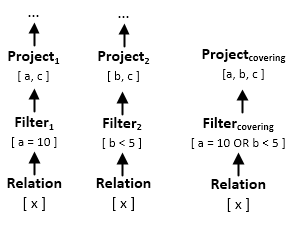
\includegraphics[scale=0.75]{figures/covering}
	\caption{Building covering subexpression example. The first and second trees are two SEs. The third tree is the CE}
	\label{fig:covering}
\end{figure}
%%%%%%%%%%%%%%%%%%%%%%%%%%%%%%%%%%%%%%%%%%%%%%%%%%%%%%%%%%%%%%%%%%%%%%%%%%%%%%%

%%%%%%%%%%%%%%%%%%%%%%%%%%%%%%%%%%%%%%%%%%%%%%%%%%%%%%%%%%%%%%%%%%%%%%%%%%%%%%%
\subsubsection{Sharing versus not sharing}
\label{sec:sharing-vs-notsharing}
To measure the benefit of sharing SEs, we consider the case where only one group of n SEs was identified among the input queries. That means one CE can be built to cover those expressions. We first compare the cost between two approaches: with and without our optimization. We use the notation $C_{E}^{se}$ and $C_{E}^{ce}$ to denote the executing costs of SE $se$ and CE $ce$. $C_{W}^{ce}$ and $C_{R}^{ce}$ are the costs of materializing (writing) the result of CE $ce$ to RAM and retrieving (reading) it back. $C_{COMP}^{se}$ indicates the cost of using the CE to answer the SE $se$.

Given a group of n SEs detected in phase 1, the cost of executing them without optimization can be computed by summing all individual executing costs: $C = \sum_{i=1}^{n}C_{E}^{se_i}$. In contrast, by building a CE and use it as a \emph{cache plan}, this cost becomes: 
$C^* = C_{E}^{ce} + C_{W}^{ce} + \sum _{i=1}^{n}(C_{R}^{ce} + C_{COMP}^{se_i})$. 
CE will be executed and materialized to RAM once. Then the result is read back to answer each individual SE. Only when $C^* < C$, caching brings some benefit in reducing the total job's running time. $C_{E}^{se}$, $C_{E}^{ce}$ and $C_{COMP}^{se_i}$ can be estimated by using cost estimation. $C_{W}^{ce}$ is proportional to the cache size of $ce$, which can be estimated using cardinality estimation. $C_{R}^{ce}$, the cost of reading the cached result of $ce$, is expected to be relatively small. We define the profit $P = (C^*-C)$ which is the profit of using a $ce$ as the cache plan.

%%%%%%%%%%%%%%%%%%%%%%%%%%%%%%%%%%%%%%%%%%%%%%%%%%%%%%%%%%%%%%%%%%%%%%%%%%%%%%%


%%%%%%%%%%%%%%%%%%%%%%%%%%%%%%%%%%%%%%%%%%%%%%%%%%%%%%%%%%%%%%%%%%%%%%%%%%%%%%%
\subsubsection{Pruning bad SEs}
\label{sec:se-prune}
The size of the \emph{cache plans} not only affects the memory occupation but also brings materializing costs, and CEs are potential candidates for \emph{cache plans} selection. Intuitively, good candidates of \emph{cache plans} are those have the output sizes satisfy the memory constraint while (1) have high frequent of use and/or (2) are expensive to (re)compute, for example producing small amount of output while reading and computing a large amount of input data. Thus, cheap SEs (fast to compute) and heavy SEs (their output exceeds the memory capacity) should be eliminated early from consideration of sharing. We rather compute them from scratch than just gain a small benefit while paying a big cost in caching a large amount of data. We propose the following threshold-based rules to quickly remove bad sharing candidates:

For each group $g_i=\{SE_j\}_{j=1}^n$

\textbf{Rule 1 - prune small profit SE group}\\
If $maximum\_profit < T1$ then eliminate $g_i$ from sharing. Let $SE_{min}$ be the similar expression in $g_i$ having smallest execution cost. We define $maximum\_profit=\sum_{j=1}^{n}C_{E}^{se_j} - (C_{E}^{se_{min}} + C_{W}^{se_{min}} + n*C_{R}^{se_{min}})$. $T1$ is a predefined threshold.

\textbf{Rule 2 - prune SEs having big output}\\
For each $SE_j$ in $g_i$, remove $SE_j$ from $g_i$ if $output\_size(SE_j) > T2$. Then $g_i$ will be eliminated if $|g_i| < 2$ (we need at least 2 SEs to make them share the computation). $T2$ is a predefined threshold.
%%%%%%%%%%%%%%%%%%%%%%%%%%%%%%%%%%%%%%%%%%%%%%%%%%%%%%%%%%%%%%%%%%%%%%%%%%%%%%%

%%%%%%%%%%%%%%%%%%%%%%%%%%%%%%%%%%%%%%%%%%%%%%%%%%%%%%%%%%%%%%%%%%%%%%%%%%%%%%%
\subsubsection{Independent SE groups}
Check for independent groups

Eliminate the worse (heuristics)

Generate final classes for multiple choice Knapsack in next phase.

%%%%%%%%%%%%%%%%%%%%%%%%%%%%%%%%%%%%%%%%%%%%%%%%%%%%%%%%%%%%%%%%%%%%%%%%%%%%%%%